\documentclass{acm_proc_article-sp}

\begin{document}

\title{LifeScope: A Multimodal Mobile Time Tracking Application}

\numberofauthors{3}
\author{
% 1st. author
\alignauthor
Luca Foschini\\
       \affaddr{University of California, Santa Barbara}\\
       \email{foschini@cs.ucsb.edu}
% 2nd. author
\alignauthor
Danny Iland\\
       \affaddr{University of California, Santa Barbara}\\
       \email{iland@cs.ucsb.edu}
% 3rd. author
\alignauthor 
Ian Whitfield\\
       \affaddr{University of California, Santa Barbara}\\
       \email{ianwhitfield@cs.ucsb.edu}
}

\def\LS{{\tt LifeScope}}

\maketitle
\begin{abstract}
In this paper, we present \LS, an Android app that tracks and identifies daily activity of a user of a handheld device.
\LS harness input from a variety of sensors to detect what activity is being performed by the user. Detected activities are then summarized on a time and geographic scale chosen by the user.
In what follows, we describe the architecture of \LS, and discuss our design choices. Finally, we present an evaluation of \LS in terms of detection accuracy and battery usage.

% Need one reference to make it compile properly.
\cite{Lamport:LaTeX}.
\end{abstract}

% A category with the (minimum) three required fields
\category{H.5}{Information Systems}{INFORMATION INTERFACES AND PRESENTATION}
\terms{Mobile computing, context-aware, multimodal interaction}

\section{Introduction}
The modern smartphone  

- new possibilities of activity monitoring given by sensor fusion, possibility to connect to other body sensors

- gateway to user activities.

- allow monitor your activity, new concept of "quantify self". Unlock a huge amount of data and knowledge about user activities

- future possibility to program actions in response to detected activities

%%%%%%%%%%%%%%%%%%%%%%%%%%%%%%%%%%%%%%%%%%%%%%%%%%%%%%%%%%%%%%%

\section{Related Work}
There has been an increasing interest in the pervasive computing community about "context monitoring" and "context recognition" in mobile devices. Context recognition applications are able to identify a person's activity at a particular point in time~\cite{CONTEXTRECOGNITIONSTUFF}. A recent development of the context recognition is the idea of context monitoring~\cite{MOBICON_PAPER} which involves execution of complex multi-step operations and correlating the output of different sensors.

While research has focused on defining an API/middleware to provide context to different applications as to minimize resource-intensive sensor querying, such systems are not freely available.

Among open source and readily usable we find The funf Open Sensing Framework~\cite{FUNF}  of MIT Media Lab, provides interface to query sensors blah. Sensor managed as shared resources as to minimize polling, etc...

Finally, among the end-applications that use sensor-rich framework for context recondition we must mention the recent MS on{X}~\cite{ONX}. Description....

The development of the two sides of context aware applications, sensor framework like funf on one hand, the applications that use it, like on{X} on the other are very recent and changing every day...
Expectation that lots is going to happen in the next few years...

%%%%%%%%%%%%%%%%%%%%%%%%%%%%%%%%%%%%%%%%%%%%%%%%%%%%%%%%%%%%%%%

\section{Approach and Implementation}
In LifeScope, we use the generalization that people go places to perform actions. For example, the user might go to the gym and work out, and then return home to work on a project, and finally go to sleep.  In LifeScope, this series of events would be modeled as two places, with one action at the first location and two actions at the second location. While this model does not support actions that span multiple places, we believe that it adequately models the majority of use cases and greatly simplifies the rest of our implementation. 

Our approach can then be broken down into two main components: identifying places that a user travels to and then, once at a place, identifying the actions performed.

\subsection {Location Management}

Since activities take place at specific locations an important first step was to be able to accurately determine a user's current location and detect when they move to a new location. For this we decided to use two approaches. We use Alohar, a third-party API, which uses Wi-Fi SSIDs (and their associated signal strengths) combined with GPS to accurately and continuously record a phone�s position. Alohar runs as a service in the background, and launches on startup. Alohar also performs filtering and analysis of this location data, in order to provide a rich API, which can be easily queried. A query for locations visited in a specific time range results in a list of Alohar UserStays, which consist of a centroid latitude and longitude, a time of arrival and departure, and several candidate Place objects, each with a name, address, and category. We map these UserStays in the Locations tab, and display the best guess Place data.

It is important to note that Alohar UserStays are created only when multiple location readings indicate a stable centroid latitude and longitude. In our experiments, it took Alohar 5-10 minutes to create a UserStay after arriving at an indoor location with many nearby access points. Since we wish to allow arbitrary location-based detectors, we also register a listener for Google's Location Service, and log the current latitude and longitude at 30 second intervals. This allows detectors to set location triggers, and locations to be recognized even if they are ephemeral in nature, and would not create an Alohar User Stay. 

\subsection {Action Recognition}
The core component of our activity recognition system is the Detector, each of which activates in response to a specific, predefined condition. The user groups configured instances of Detectors into actions with descriptive titles such as "working on CS 290". When all the detectors for an action are active when the user is at a location, it is determined that the user was performing that action at that location. The Detectors are backed by Data Sources, which maintain databases of events that may cause a Detector to activate. A Data Source may store its data locally, or may be acting as a proxy for a cloud service API such as Google Calendar. Each Detector queries one or more data sources to determine if it is active.

\subsection {Application Architecture}
Due to its widespread adoption and rich application API (especially for background activity), we decided to implement LifeScope as a user-installable application (``App'') for the Android smartphone operating system.

Internally, our application is structured as a pair of always-running Service components with a number of standalone Activity components that connect to them. The first Service component hosts the currently enabled Detectors and Data Sources. It allows Data Sources to collect data from device sensors and cloud APIs even when the user is not actively using the application. Client Activity components may connect to this Service to register new actions (which contain Detector instances), or determine which of the registered actions has been performed at a given location.

The second Service contains the Alohar and Google location tracking systems and, as with the first service, allows them to continue running in the background and log events when the user transitions to a new location.

Events from both the Data Sources and location trackers are stored in SQLite databases for simple querying from Detectors and, if desired, custom queries by the user from another SQLite client.

\begin{figure}
\begin{center}
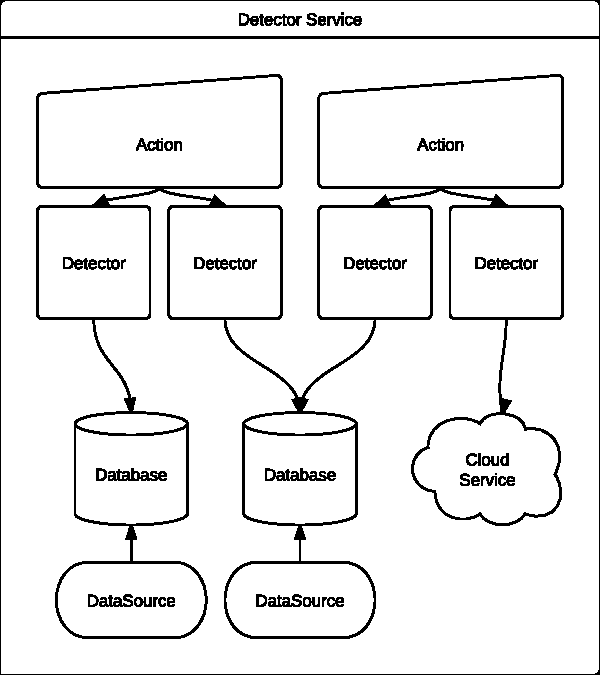
\includegraphics[width=3in]{arch}
\caption{
Architecture of the Detector Service, which stores registered Actions and Detectors and allows the Data Sources to run in the background collecting data.
}
\label{figure:voice}
\end{center}
\end{figure}

\subsection{Detectors Implemented}

talk about the quantized levels that the data sources use
why we write every minute
the moving average with two thresholds in the workout detector to eliminate jitter


\subsection {User Interface}
The user interface was designed to follow Android best-practices and features a number of different interaction modes. As is typical for a modern smartphone application, basic interaction with the application is performed with a simple tapping interface. 

A major component of our application is the interactive map view, which shows places the user has visited (and stayed at for a period of at least 5 minutes). The map view supports a richer set of touch interaction modes with dragging to pan the map, pinching to zoom the map and, after first selecting a menu option, dragging to adjust the position of existing place markers.

As entering text is often a cumbersome task on smartphones without actual keyboards all text entry fields within the application have been extended with a voice input button, Figure \ref{figure:voice}.

\begin{figure}
\begin{center}
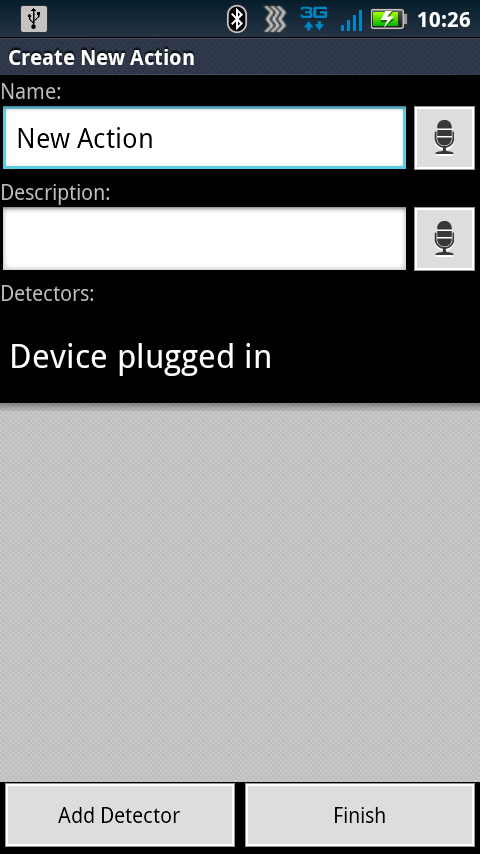
\includegraphics[height=2.5in]{voiceinput}
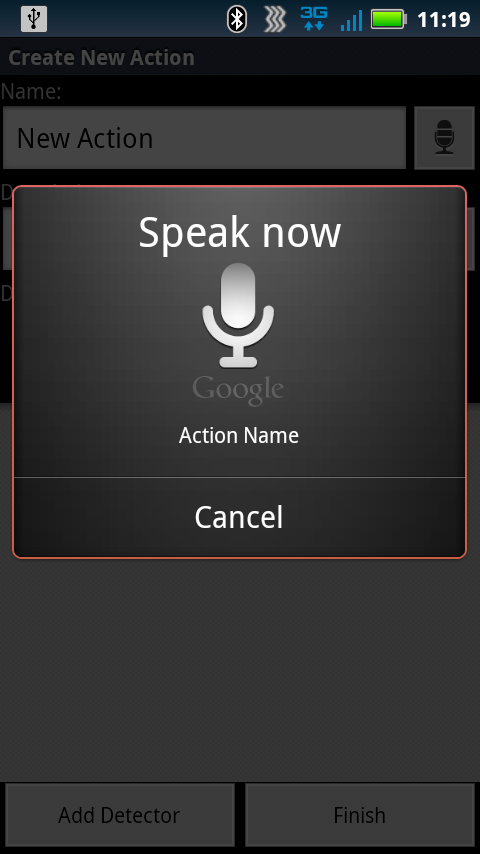
\includegraphics[height=2.5in]{voiceinput2}
\caption{
Creating a new action. All text fields are extended with a voice input button with a microphone icon. Tapping a voice input button records, recognizes, and then populates the corresponding text field with the user's speech. 
}
\label{figure:voice}
\end{center}
\end{figure}

\begin{figure}
\begin{center}
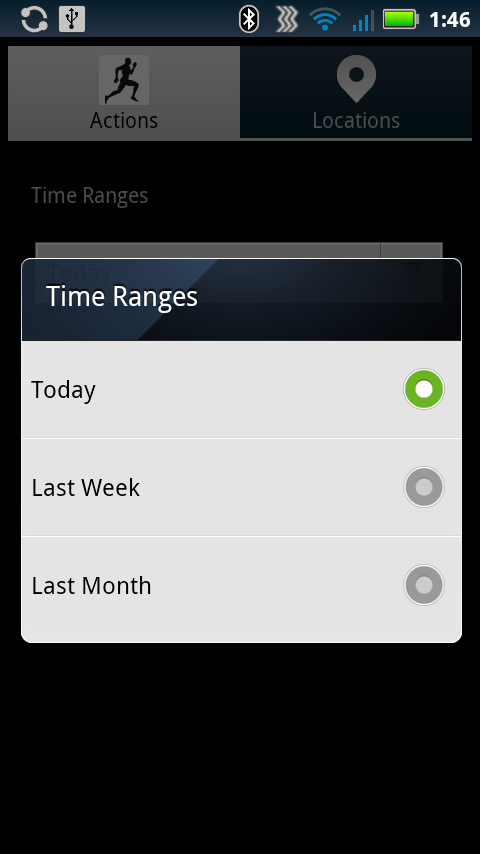
\includegraphics[height=2.5in]{ranges}
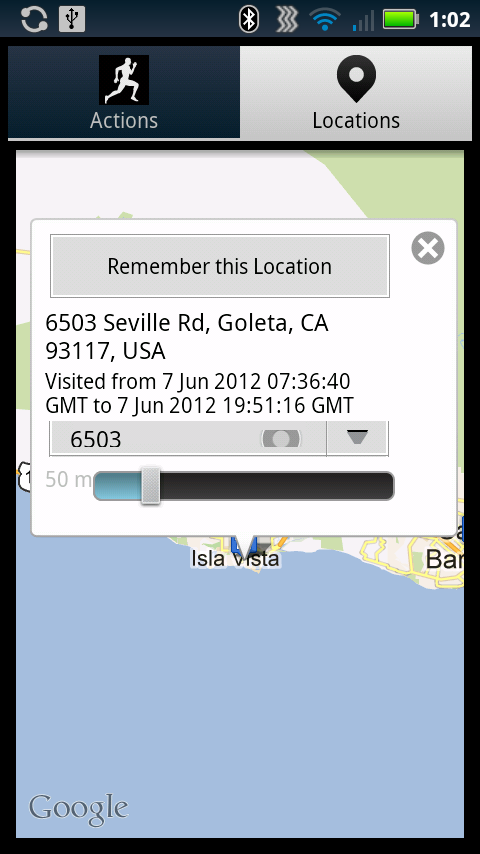
\includegraphics[height=2.5in]{map1}
\caption{
The two main views of the application. TODO(Luca): Caption
}
\label{figure:voice}
\end{center}
\end{figure}

%%%%%%%%%%%%%%%%%%%%%%%%%%%%%%%%%%%%%%%%%%%%%%%%%%%%%%%%%%%%%%%

\section{Assessment}

It's difficult to evaluate the effectiveness of \LS as a whole without an in-depth user studies. Therefore, we focus on evaluating specific aspects of the inner workings of \LS.

\subsection{Power Consumption}
An important design consideration for smartphone applications is their impact on battery life. If an application consumes so much power that the device prematurely runs out of power, the user will likely uninstall the application. Mobile context monitoring is an inherently expensive activity, in terms of power usage. The GPS and WiFi radios must remain on for accurate position estimates, and CPU cycles are required for analyzing data samples taken from the device's on-board sensors. For the application to build a complete model of the user's activities, it must remain running in the background and even when the phone is asleep. 

To minimize power draw \LS disables Data Sources that are not currently required by any registered Detectors. For example, if there are no detectors that need readings from the accelerometer sensor, its Data Source will not be activated and no samples will be read from the accelerometer. When the user adds an action containing a Detector that requires information from the accelerometer Data Source, it will be started automatically. Thus, the exact power usage of the application depends on how the user has configured it.

To understand how different detectors affect power usage, we performed a series of experiments. In each experiment one Data Source was enabled, and then the phone was left in its sleep state for a fixed period of time. The battery level was measured before and after each experiment to determine the effect of each Data Source on the device's battery life.

\subsection{Location Accuracy}
TODO: Danny might want to add something here


%%%%%%%%%%%%%%%%%%%%%%%%%%%%%%%%%%%%%%%%%%%%%%%%%%%%%%%%%%%%%%%

\section{Conclusions and Future Work}
In this paper we present \LS an android app that allow a user of a handheld device to track and analyze their daily activity. \LS leverages input from a variety of sensors to determine what activity is being currently performed by the user. \LS allows then provides methods to summarize all of the user's activities on a given timeframe or geographic area.
We evaluated the accuracy of sensor identification for the geographic location and the battery usage of the app. We found that the battery usage in the case \LS is set up to monitor a reasonable amount of activities is negligible. Also, location accuracy is good enough (?? will fix it when I read Danny's section)
As far as the future work is concerned, we recognize that a system like \LS would benefit of many additional features if it were to be released to the general public. 
First of all, more detectors are needed to be able to describe a richer set of activities.
Then, a mechanism to guide/correct the detection of actions would be beneficial, for which the user can review/change the detected action. This is especially true if such a mechanism allowed the app to learn from the user corrections.
Finally, another possible improvement could be the ability to specify actions not only using ittt rules, but by recording the sensor inputs while performing an activity to be recognized later, and then try to match such input to future sensor readings. Such a "record activity" feature is highly desirable to minimize user interaction, but is hard to implement, as current research in activity identification is still struggling with identifying vary basic actions such as running/biking/driving ~\cite{STUFFONCOURSEHOMEPAGE}

%%%%%%%%%%%%%%%%%%%%%%%%%%%%%%%%%%%%%%%%%%%%%%%%%%%%%%%%%%%%%%%

\bibliographystyle{abbrv}
\bibliography{bibliography}  % sigproc.bib is the name of the Bibliography in this case

% That's all folks!
\end{document}
